%%%% Proceedings format for most of ACM conferences (with the exceptions listed below) and all ICPS volumes.
\documentclass[sigconf]{acmart}
%%%% As of March 2017, [siggraph] is no longer used. Please use sigconf (above) for SIGGRAPH conferences.

%%%% Proceedings format for SIGPLAN conferences 
% \documentclass[sigplan, anonymous, review]{acmart}

%%%% Proceedings format for SIGCHI conferences
% \documentclass[sigchi, review]{acmart}

%%%% To use the SIGCHI extended abstract template, please visit
% https://www.overleaf.com/read/zzzfqvkmrfzn


%%%%%%%%%%%%%%%%%%%%%%%%%%%%%%%%%%%%%%%%%%%%%%%%%%%%%%%%%%%%%%%%%%%%%%%%%%%%%%%%%%%%%%%%%%%%%%%%%%%%%%%%%%%%%%%%%%%%%%%%%%%%%%%%%%%%%%%%%%%%%%%%%%%%%%%%%
% PACKAGES
%%%%%%%%%%%%%%%%%%%%%%%%%%%%%%%%%%%%%%%%%%%%%%%%%%%%%%%%%%%%%%%%%%%%%%%%%%%%%%%%%%%%%%%%%%%%%%%%%%%%%%%%%%%%%%%%%%%%%%%%%%%%%%%%%%%%%%%%%%%%%%%%%%%%%%%%%
\usepackage{booktabs} % For formal tables
%% perso packages:
\usepackage{epstopdf}
\usepackage{microtype}
\usepackage{tabularx}
\usepackage{multirow}
%\usepackage{arydshln}
\usepackage{subfig}
\usepackage{balance}
\usepackage{caption}
\usepackage{graphicx}

%%%%%%%%%%%%%%%%%%%%%%%%%%%%%%%%%%%%%%%%%%%%%%%%%%%%%%%%%%%%%%%%%%%%%%%%%%%%%%%%%%%%%%%%%%%%%%%%%%%%%%%%%%%%%%%%%%%%%%%%%%%%%%%%%%%%%%%%%%%%%%%%%%%%%%%%%
% DOCUMENT's Identification
%%%%%%%%%%%%%%%%%%%%%%%%%%%%%%%%%%%%%%%%%%%%%%%%%%%%%%%%%%%%%%%%%%%%%%%%%%%%%%%%%%%%%%%%%%%%%%%%%%%%%%%%%%%%%%%%%%%%%%%%%%%%%%%%%%%%%%%%%%%%%%%%%%%%%%%%%
% Copyright
%\setcopyright{none}
%\setcopyright{acmcopyright}
%\setcopyright{acmlicensed}
\setcopyright{rightsretained}
%\setcopyright{usgov}
%\setcopyright{usgovmixed}
%\setcopyright{cagov}
%\setcopyright{cagovmixed}


% DOI
\acmDOI{10.475/123_4}

% ISBN
\acmISBN{123-4567-24-567/08/06}


%%%%%%%%%%%%%%%%%%%%%%%%%%%%%%%%%%%%%%%%%%%%%%%%%%%%%%%%%%%%%%%%%%%%%%%%%%%%%%%%%%%%%%%%%%%%%%%%%%%%%%%%%%%%%%%%%%%%%%%%%%%%%%%%%%%%%%%%%%%%%%%%%%%%%%%%%
% CONFERENCE
%%%%%%%%%%%%%%%%%%%%%%%%%%%%%%%%%%%%%%%%%%%%%%%%%%%%%%%%%%%%%%%%%%%%%%%%%%%%%%%%%%%%%%%%%%%%%%%%%%%%%%%%%%%%%%%%%%%%%%%%%%%%%%%%%%%%%%%%%%%%%%%%%%%%%%%%%
%Conference
\acmConference[ICMR 2018]{ACM Yokohama conference}{June 2018}{Yokohama, Japan} 
\acmYear{2018}
\copyrightyear{2018}

\acmArticle{4}%??
\acmPrice{15.00}%??

%%%%%%%%%%%%%%%%%%%%%%%%%%%%%%%%%%%%%%%%%%%%%%%%%%%%%%%%%%%%%%%%%%%%%%%%%%%%%%%%%%%%%%%%%%%%%%%%%%%%%%%%%%%%%%%%%%%%%%%%%%%%%%%%%%%%%%%%%%%%%%%%%%%%%%%%%
\begin{document}
%%%%%%%%%%%%%%%%%%%%%%%%%%%%%%%%%%%%%%%%%%%%%%%%%%%%%%%%%%%%%%%%%%%%%%%%%%%%%%%%%%%%%%%%%%%%%%%%%%%%%%%%%%%%%%%%%%%%%%%%%%%%%%%%%%%%%%%%%%%%%%%%%%%%%%%%%

%%%%%%%%%%%%%%%%%%%%%%%%%%%%%%%%%%%%%%%%%%%%%%%%%%%%%%%%%%%%%%%%%%%%%%%%%%%%%%%%%%%%%%%%%%%%%%%%%%%%%%%%%%%%%%%%%%%%%%%%%%%%%%%%%%%%%%%%%%%%%%%%%%%%%%%%%
% TITLE
%%%%%%%%%%%%%%%%%%%%%%%%%%%%%%%%%%%%%%%%%%%%%%%%%%%%%%%%%%%%%%%%%%%%%%%%%%%%%%%%%%%%%%%%%%%%%%%%%%%%%%%%%%%%%%%%%%%%%%%%%%%%%%%%%%%%%%%%%%%%%%%%%%%%%%%%%
\title{Annotating, understanding, and predicting long-term video memorability}
\titlenote{Produces the permission block, and copyright information}
\subtitle{Extended Abstract}
\subtitlenote{The full version of the author's guide is available as
\texttt{acmart.pdf} document}

%%%%%%%%%%%%%%%%%%%%%%%%%%%%%%%%%%%%%%%%%%%%%%%%%%%%%%%%%%%%%%%%%%%%%%%%%%%%%%%%%%%%%%%%%%%%%%%%%%%%%%%%%%%%%%%%%%%%%%%%%%%%%%%%%%%%%%%%%%%%%%%%%%%%%%%%%
% AUTHORS
%%%%%%%%%%%%%%%%%%%%%%%%%%%%%%%%%%%%%%%%%%%%%%%%%%%%%%%%%%%%%%%%%%%%%%%%%%%%%%%%%%%%%%%%%%%%%%%%%%%%%%%%%%%%%%%%%%%%%%%%%%%%%%%%%%%%%%%%%%%%%%%%%%%%%%%%%
\author{Romain Cohendet}
%\authornote{}
%\orcid{1234-5678-9012}
\affiliation{%
	\institution{Technicolor}
	\streetaddress{}
	\city{Rennes} 
	\state{France} 
	\postcode{}
}
\email{romain.cohendet@technicolor.com}

\author{Karthik Yadati}
\affiliation{%
	\institution{University of Delft}
	\streetaddress{}
	\city{Delft} 
	\state{} 
	\postcode{}
}
\email{N.K.Yadati@tudelft.nl}

\author{Ngoc Khanh Duong}
\affiliation{%
	\institution{Technicolor}
	\city{Rennes} 
	\country{France}}
\email{Quang-Khanh-Ngoc.Duong@technicolor.com}

\author{Claire-Helene Demarty}
\affiliation{%
	\institution{Technicolor}
	\city{Rennes}
	\country{France}
}
\email{Claire-Helene.Demarty@technicolor.com}

% The default list of authors is too long for headers.
\renewcommand{\shortauthors}{R. Cohendet et al.}

%%%%%%%%%%%%%%%%%%%%%%%%%%%%%%%%%%%%%%%%%%%%%%%%%%%%%%%%%%%%%%%%%%%%%%%%%%%%%%%%%%%%%%%%%%%%%%%%%%%%%%%%%%%%%%%%%%%%%%%%%%%%%%%%%%%%%%%%%%%%%%%%%%%%%%%%%
% ABSTRACT
%%%%%%%%%%%%%%%%%%%%%%%%%%%%%%%%%%%%%%%%%%%%%%%%%%%%%%%%%%%%%%%%%%%%%%%%%%%%%%%%%%%%%%%%%%%%%%%%%%%%%%%%%%%%%%%%%%%%%%%%%%%%%%%%%%%%%%%%%%%%%%%%%%%%%%%%%
\begin{abstract}
Following the interest of these last years for image memorability prediction, video memorability has recently attracted attention of researchers.
The growing number of video shared everyday forces us to find new way to deal with them to make the most relevant their occurrence in our everyday lives.

Recently, two studies have tried to predict video memorability ; however, the immaturity of this work is obvious.
In particular, none of these studies on images nor videos tried to measure 'very' long-term memory: they just measured the memory of items some minutes after the memory encoding.
In this paper, we propose a dataset of 700 videos annotated with memorability scores corresponding to real long-term memory.
We discuss in details the method and the proponents.
We then propose a model to predict memorability of videos and test it on the available dataset of images and videos.
% Our approach improves over current memorability methods in this task.
The material -- videos plus theirs memorability scores -- is made accessible for researchers.
\end{abstract}

%%%%%%%%%%%%%%%%%%%%%%%%%%%%%%%%%%%%%%%%%%%%%%%%%%%%%%%%%%%%%%%%%%%%%%%%%%%%%%%%%%%%%%%%%%%%%%%%%%%%%%%%%%%%%%%%%%%%%%%%%%%%%%%%%%%%%%%%%%%%%%%%%%%%%%%%%
%% NEW ACM TAXONOMY to categorise ACM article
%%%%%%%%%%%%%%%%%%%%%%%%%%%%%%%%%%%%%%%%%%%%%%%%%%%%%%%%%%%%%%%%%%%%%%%%%%%%%%%%%%%%%%%%%%%%%%%%%%%%%%%%%%%%%%%%%%%%%%%%%%%%%%%%%%%%%%%%%%%%%%%%%%%%%%%%%
\begin{CCSXML}
	<ccs2012>
	<concept>
	<concept_id>10010520.10010553.10010562</concept_id>
	<concept_desc>Computer systems organization~Embedded systems</concept_desc>
	<concept_significance>500</concept_significance>
	</concept>
	<concept>
	<concept_id>10010520.10010575.10010755</concept_id>
	<concept_desc>Computer systems organization~Redundancy</concept_desc>
	<concept_significance>300</concept_significance>
	</concept>
	<concept>
	<concept_id>10010520.10010553.10010554</concept_id>
	<concept_desc>Computer systems organization~Robotics</concept_desc>
	<concept_significance>100</concept_significance>
	</concept>
	<concept>
	<concept_id>10003033.10003083.10003095</concept_id>
	<concept_desc>Networks~Network reliability</concept_desc>
	<concept_significance>100</concept_significance>
	</concept>
	</ccs2012>  
\end{CCSXML}

%\ccsdesc[500]{Computer systems organization~Embedded systems}
%\ccsdesc[300]{Computer systems organization~Redundancy}
%\ccsdesc{Computer systems organization~Robotics}
%\ccsdesc[100]{Networks~Network reliability}

%%%%%%%%%%%%%%%%%%%%%%%%%%%%%%%%%%%%%%%%%%%%%%%%%%%%%%%%%%%%%%%%%%%%%%%%%%%%%%%%%%%%%%%%%%%%%%%%%%%%%%%%%%%%%%%%%%%%%%%%%%%%%%%%%%%%%%%%%%%%%%%%%%%%%%%%%
% KEYWORDS
%%%%%%%%%%%%%%%%%%%%%%%%%%%%%%%%%%%%%%%%%%%%%%%%%%%%%%%%%%%%%%%%%%%%%%%%%%%%%%%%%%%%%%%%%%%%%%%%%%%%%%%%%%%%%%%%%%%%%%%%%%%%%%%%%%%%%%%%%%%%%%%%%%%%%%%%%
\keywords{Video memorability, Long-term memory, Measurement protocol, Memorability scores, Deep learning, Multimedia information retrieval}

%%%%%%%%%%%%%%%%%%%%%%%%%%%%%%%%%%%%%%%%%%%%%%%%%%%%%%%%%%%%%%%%%%%%%%%%%%%%%%%%%%%%%%%%%%%%%%%%%%%%%%%%%%%%%%%%%%%%%%%%%%%%%%%%%%%%%%%%%%%%%%%%%%%%%%%%%
%% ABOUT ICMR'2018 article...
%%%%%%%%%%%%%%%%%%%%%%%%%%%%%%%%%%%%%%%%%%%%%%%%%%%%%%%%%%%%%%%%%%%%%%%%%%%%%%%%%%%%%%%%%%%%%%%%%%%%%%%%%%%%%%%%%%%%%%%%%%%%%%%%%%%%%%%%%%%%%%%%%%%%%%%%%
\maketitle
%if we want the text be called from there
 %\input{samplebody-conf}

%% About the ICMR article on Media retrieval with video memorability
	% focus on "Multimedia content-based retrieval"
	% Length: from 6 to 8 pages + 1 additional page for references (no longer distinction between long and short papers)
	% Submission deadline: 2018/01/20
	% Contributions addressing the challenges of large-scale search and user behavior analysis are especially welcome

%%%%%%%%%%%%%%%%%%%%%%%%%%%%%%%%%%%%%%%%%%%%%%%%%%%%%%%%%%%%%%%%%%%%%%%%%%%%%%%%%%%%%%%%%%%%%%%%%%%%%%%%%%%%%%%%%%%%%%%%%%%%%%%%%%%%%%%%%%%%%%%%%%%%%%%%%
\section{INTRODUCTION}%nb of sections %2 PAGES
%%%%%%%%%%%%%%%%%%%%%%%%%%%%%%%%%%%%%%%%%%%%%%%%%%%%%%%%%%%%%%%%%%%%%%%%%%%%%%%%%%%%%%%%%%%%%%%%%%%%%%%%%%%%%%%%%%%%%%%%%%%%%%%%%%%%%%%%%%%%%%%%%%%%%%%%%
%citer Qomex
%citer Deep learning emotional images bias
\paragraph{Opening} % oder Ok
To deal with the constant increase in shared videos, we must imagine new ways to organize -- in particular, to retrieve -- videos with the aim of improving the relevance of their occurrences in our every day lives.
Contrary to other metrics used to quantify image of video importance, such as aesthetics or interestingness, whose corresponding ground truths corresponds to subjective judgments, memorability can be objectively measured by a memory test.
As such, memorability can be regarded as a particularly relevant element to help us picking a video among several ones.

\paragraph{The field of video memorability is very immature}
%from images to video memorability
The image memorability prediction challenge has attracted increasing attention from the seminal work of Isola \textit{et al.} released in 2001 \cite{isola_2011_makes}.
Recently, models achieved very good results with the introduction of deep learning to address the challenge \cite{khosla_2015_understanding,baveye_2016_deep}% plus papier Hammad
As a result of this success, the search field has been extended to videos.
Video memorability prediction is however a very new field, and there are only two studies, to our knowledge, that address this issue \cite{han_2015_learning,shekhar_2017_show}.

At least two important problems could explained this scarcity of studies.
Firstly, protocols used in the existing studies are not smart enough, but are easily critisizeable.
Secondly, authors didn't make their data accessible for community, so no database exist.

\subsection{Problem 1: The problem of the weakness of the studies}
%%% Critiques of previous studies %%%

\paragraph{Critics of Han et al.}
The previous attempt at creating memorability video dataset first approach to model video memorability had been propose by \cite{han_2015_learning}. 
This first attempt is a "strange" adaptation of \cite{isola_2011_makes} protocols.

% A memory game of 12 hours
- Firstly, the authors call their task a "memory game" as Isola \textit{et al.}. If it were justified for Isola et al., 2011, la tâche dure pour 1 unique participant environ 12 heures. The authors do not provide this time, but it cans be deduced from the by the following calculation:


Thenks to this maneer, participants obtained a dataset of videos with only 20 participants (we don\'t know if they are student or payed).




répatit sur 10 jours diffférens (5 pour les phases dapprentissage + 5 pour les phase de mesure de la mémoire).

uen autre aberration e





%critique of Shekhar et al.
In \cite{shekhar_2017_show}, 
- des questions pas forcément aussi faciles/diffilec entre les vidéos, qui peuvent expliquer leur 

Enfin, dans les deux études précédentes, la congruence inter-humaine, minimum nécessaire pour s'assurer de la cohérence des données et avoir une base de comparaison pour les modèles, n'a pas été fournie.


%Lasting long-term memory for IMAGES - critic of Isola et al.
on comprend les auteur d'avoir agit ainsi pour consituter une base de grand ampleur (Khosla et al.)
It is long-term memory a proprement parlé because.
but memories evolove in l-g mem
=> Ebbinghaus curve
So memorabilities of souvenirs can change after a certain delays
%as proposed in [ma thèse] 
%Memorability continue to evolve in long-term memory --> Ebbinghaus -- or more recent similar -- curve
%Memorability image/videos in computer vision never interested in REAL long-term memory
%We want to correct this problem by proposing a new way to measure memorability.
% saut de la tâche d'apprentissage (remplacée par le questionnaire)
% To sum up, we want to obtain the "long-lasting memorability" of the videos


\paragraph{Problem 2: No existing database}
%there is no database
=> Dataset non disponible pour les deux études.

The fact that there exist no dataset to modeling video memorability is the most serious obstacle which prevent video memorability prediction to take off.
This should be the very first goal of pioneers of this new research field: to provide data to community.
For images, the pioneers created and made downloadable such a database \cite{isola_2011_makes}, which enable to made image memorability research flourishing.
The second released database, far larger, launched new possibility for deep learning and enable to obtained the aforementioned really good results \cite{khosla_2015_understanding}.
Nous pouvons parier qu'il en sera de même pour le cham de la mémorabilité des vidéos.

%it's not easy to construct the first dataset
The establishment of a dataset, in particular of the first dataset of this kind, may not be self-evident.

Elle nécessite de définir les points cardinaux qui vont guider – et contraindre – les chercheurs qui utiliseront ces premières données disponibles.

Pour preuve, l'influence considérable qu'Isola et al. (puis Khosla et al., de la même équipe, avec leur base de données beaucoup plus conséquente rendue disponible en 2015) ont eu sur les études réalisées dans leur sillage : jusqu'à aujourd'hui, la quasi-totalité des études ayant porté sur la mémorabilité des images ont adopté – avec les bases de données de ces auteurs – leurs définitions de la mémorabilité.

Or, la manière dont les auteurs ont mesuré la mémorabilité des images, qui n'est pratiquement jamais rediscutée, n'est qu'une des manières de procéder.

Aussi, si les modèles de prédiction de la mémorabilité des images ont obtenu d'excellents résultats (très proches de ceux qu'on obtiendrait en inférant des résultats d'un groupe d'observateur les résultats d'un autre groupe d'observateurs), qu'est-ce que ces modèles prédisent si bien, en fait ? 

	%Difficulty: define video unity; complexity of the videos compare to images
	Videos are more complex than images. Contrary to images, videos do not constitute clearly defined units, but have supplementary dimensions -- sound and movement -- that makes difficult the definition of what a video is.
	%from ahn et al. Videos contain a synthesis of visual, aural, textual, and 	motion information and generally convey relatively richer 	media content than images.


%Conclusion paragraph: we want to contribute to the protocol creation by proposing one method
Aussi cette étude veut participer à réfléchir aux protocoles qui pourraient être employée pour contituer à l'avenir à un protocole de plus grande envergure.




\paragraph{Goals of our study}
%link the two reasons precebndtky evoque
These two reasons are linked. They give us our priority: build a dataset and define a protocol to do that.
This dataset -- and a fortiori the protocol -- should avoid the drawbacks of previous work in video and image memorability.
%in image memorability, difficultys come from que'elle ont justement utilisés ces bases de données.

%2 resaons => our goal of our study => correct these drawbacks
=> To propose a new protocol to collect data/for annotation
=> To propose a dataset
=> The dataset will have "lasting" long-term memorability annotations
We want our work would benefit to video but also to image memorability. 


%Ainsi, puisque les limitations d'un protocole destiné à collecter des données tendent à se répercuter dans les travaux qui utilisent celles-ci, un protocole destiné à constituer la base nécessaire pour répondre au défi de la prédiction de la mémorabilité des vidéos devra répondre à de strictes exigences de qualité. La qualité des données obtenues, primordiale, nécessite une connaissance profonde des phénomènes que ces données sont censées refléter. La mémoire étant un phénomène étudié (depuis plus d'un siècle) par la psychologie, et les modèles computationnels permettant de l'inférer des caractéristiques des vidéos appartenant au domaine de l'informatique, l'approche transdisciplinaire semble la plus adaptée dans ce cas. 

%%%%%%%%%%%%%%%%%%%%%%%%%%%%%%%%%%%%%%%%%%%%%
\paragraph{Secondary goals}
%%% OTHER INTERSTING RESULTS
%will depend on our results
%\paragraph{Exploiting response time for memorability scores}
%D'autre part, nous voulons également estimer si le temps de réponse à un effet sur la mémorabilité, c'est-à-dire qu'il pourrait être pris en compte pour corriger les scores calculer. Note hypothèse est que, plus les participants sont sûrs d'eux, plus ils vont tendre à répondre rapidement. Att!! peut pas être tester directement : We hypothesized that the most memorable the sequence, the faster the participant will answer. Parce que les video les mieux représentés dans l'esprit sont les plus accessibles et que les participants ne veulent pas louper la préponse quand ils sont sûrs.
% Citer papiers - s'il en existe -- où les auteurs exploitent le temps de réponse pour corriger les scores de mémorabilité;

%\paragraph{Personalization of the data}
%Taking into account human factors
	%see results Logistic regression vs. SVM

il semble des dernière études qu'il serait intéressant de prendre en temps le dans le calcul de la mémorabilité [LaMem + papier sur la VM où ils prennent en compte le temps dans leurs scores]

%If results Repetition vs. memorability
The semantization that can affect long-term memorability of videos


%%%%%%%%%%%%%%%%%%%%%%%%%%%%%%%%%%%%%%%%%%%%%%%%%%%%%%%%%%%%%%%%%%%%%%%%%%%%%%%%%%%%%%%%%%%%%%%%%%%%%%%%%%%%%%%%%%%%%%%%%%%%%%%%%%%%%%%%%%%%%%%%%%%%%%%%%
\section{Construction of the dataset}
%%%%%%%%%%%%%%%%%%%%%%%%%%%%%%%%%%%%%%%%%%%%%%%%%%%%%%%%%%%%%%%%%%%%%%%%%%%%%%%%%%%%%%%%%%%%%%%%%%%%%%%%%%%%%%%%%%%%%%%%%%%%%%%%%%%%%%%%%%%%%%%%%%%%%%%%%
% Opening -- Ok for now
In this section, we describe the new protocol we propose to measure video memorability in order to collect the long-lasting memorability of the videos.
The protocol is also lighter than ordinarily since there is no need of learning step to encode the material before the recognition task, as we measure the participants' memory established prior the experiment.

The memory task involve three materials: videos sequences, questionnaire and participants.

%Insist on Contribution about the protocol (novel: how to measure long-term memory)

%%%%%%%%%%%%%%%%%%%%%%%%
\subsection{Memory task}
To measure the "real" long-term memory, we designed the recognition task presented in the figure ...%ref.
%figure Recognition task

% Targets and Fillers
The 10-sec video sequences are displayed one after another, separated by an inter-stimuli interval (ISI).

%define target and filler
Les vidéos cibles sont mêlées aux vidéos de remplissage, et le participant doit dire, pour chaque vidéo qui lui est présentée, s’il l’a déjà vue ou non.
To answer, he must press the spacebar during the displaying of the video sequences (than answer when they arrived during the 1-s inter-stimuli interval).
movies they have seen (the targets) and never seen (the fillers).
Even if the participant answers, the video continue to run until its end (to avoid the temptation of ansewering to faster finish the experiment).

"Respond ONLY if you remember the sequence AND NOT THE movie from which it comes".%reprendre phrase que j'ai écrite

%%%%%%%%%%%%%%%%%%%%%%%%
\subsection{The video sequences}
%% movies
A list of 100 movies (available with the downloadable data) was first established, for which we mixed their popularity and their genres.
The movies quality was HD 720-1080, except for ??? dvdrip movies.
orginal-english version (without subtitles) (occidental movies, except for Slumdog millionaire) %to check

%%video sequences
To constitute our dataset, we manually selected 7 video sequences of 10 seconds from each movies (for a total of 700 videos).
The sequences had to meet several criteria to be selected.
First, not to be part of the official trailers, to be sure that, if a participant report not having seen the movie, he won't have seen the sequence presented for the recognition in a trailer.
Second, we wanted our sequences to constitute "logical" units, that is to say to "protect the sens" of the videos. Indeed, semantics is linked to memorability of images \cite{isola_2014_makes}, from which we can imagine that it is also the case for videos. But, contrary to images that are clearly cut units, sequences memorability depends on the cut. To maintain a relative semantic consistency intra-sequence, the cutters were provided with the instruction to avoid to cut in the middle of a sentence, of to agglomerate very different plans together. The idea was to increase the coherence of the sequences to diminish the difficulty of he computational models to learn without impairing ther capacity to generalize.

%%Generic vs. typical
During the manual selection of the sequence, we chose 127 sequences (among the 700) we called "generic" by contrast to "typical" ones. Generic sequences are parts of the movie which do not contain any elements that would enable someone to easily guess that the sequences belong to the particular movie. The list of undesirable includes but is not limited to: scenes with recognizable famous actors (e.g. in Kill Bill, avoid the scenes with Uma Thurman, Lucy Liu, David Carradine…); scenes famous for their music, gesture... (e.g. in Kill Bill, avoid the scenes with music that enable to easily guess that the sequence comes from Kill Bill); scenes with typical elements (e.g. a spaceship or an alien from which you can easily guess that you are watching a Star Wars movie). The cutters were provided with the instructions to ask themselves the following question when choosing a generic sequence in a movie: “Could I easily guess this sequence belongs to the movie I extracted it from?” -- if the answer was yes, so don’t select this sequence.
In some movies (e.g. Kill Bill 1, Star wars, 2001 A Space Odyssey, etc.), just a few 10-sec sequences of no sequence at all were found to meet these criteria (e.g. The lord of the ring); for these movies, we don't have generic sequences.
By contrast, non-generic sequences were namely two 10-sec parts of the movie that you think are very representative of the movie (you can choose any part of the movie without restriction).
These two types of sequences should be considered in link with the instruction of the task written above (even if you know that a sequence comes from a movie, just answer if you recognize THE sequence): it is just a supplementary control (qui jour un rôle symétrique au taux de FA pour la prise de risque).

%%Indoor/Outdoor
In Isola et al., 2014, the authors showed that memorability directly correlated with color. To explain thi result, they advanced the hypothesis that the difference in memorability between indoor and outdoor scenes was due to the fact that the later tend to be less memorable that the older, and that the color tend to linked with a differences in colors, could explain this result. To validate this hypothesis, we manually annotated our 700 sequences as consisting of an indoor or outdoor scene. 


%%%%%%%%%%%%%%%%%%%%%%%%
\subsection{Questionnaire}
The targets and fillers that constitute the items of the recognition task were different for each participant.
Indeed, the video sequences viewed by a participant were selected based on response to a questionnaire presented in the figure ???
Questionnaire with the 100 movies.

%figure Questionnaire

Le nom du film, suivi de l’affiche, du nom du réalisateur et des acteurs principaux – qui permettent de s’assurer que le film que le participant a en tête est bien celui qui lui est présenté – est présenté au participant.

%Other questions associated with the questionnaire
For each movie, the participant had first to answer the following question: "Do you remember watching this movie?" -- with the fact that was madde clear that the film must been seen EN ENTIER.

If he answered "yes"
Please let us know how confident you are of having seen this movie (I am not/slightly/50\%/considerably/100\% confident)
Please let us know when did you last see this movie (<1 month; <1 year; <5 years; < 10 years; > 10 years)
Please let us know how many times did you watch this movie (once; 2-4 times; 5-9 times; 10-19 times; >20 times)

If he answered "no"
Please let us know how confident you are of NOT having seen this movie (I am not/slightly/50\%/considerably/100\% confident)
 
The goal of the confidence question was to be sure that we select video sequences from movie , to increase our certitude that target/filler were really targets/fillers.

The other two questions were used for the analysis of the results to assess factors a priori susceptible to influence video memorability. The question about the number of times the movie had been seen for us to evaluate the effect of repetition on memorization, and the question about the last time tha movie had been seen to evaluate the effect of time passage on long-term memorability, that continue to be affected in longterm memory %citer un papier de moi

%%%%%%%%%%%%%%%%%%%%%%%%
\subsection{Participants, facilities and apparatus}
%participants
??? (105) participants ($22-58$ years of age; $mean = 37.1 $; $SD = 10.4 $; $26\%$ of them female) employees of [removed for double-blind review] participated in he experiment on a volunteer basis. % Technicolor, Rennes (France). 
All participants have either normal or corrected-to-normal visual acuity.

%facilities and apparatus
%tv
%lumière tamisée
The images were displayed on a 40 inch monitor (TV SONY Bravia ???) with a display resolution of 1,920 $\times$ 1,080. The participants were comfortably seated at a distance of 150 centimeters from the screen (three times the screen height). The 1,024 $\times$ 768 images were centered on a black background; at a viewing distance of 150 cm, the stimuli subtended 18.85 degrees of vertical visual angle.

%%%%%%%%%%%%%%%%%%%%%%%%
\subsection{Procedure}
%Questionnaire part
Participants first answered the questionnaire. During the whole time, the experimenter was near the participant in case he doubt about one movie. 

%Algorithm selection
Based on the answers to the questionnaires, the algorithm selected the movies associated with the maximum certitude level (i.e. 5) to constitute  targets and fillers sets. // At the end, the algorithm selected 80 targets and 40 fillers for the participants, and place them in a random order for presentation
// The criteria of selection was the number after the response to the questionnaire the nb of annotations of the sequences, in order to harmonize the nb of annotations per video.
The sequences used as targets were selected among the sequences corresponded to the movies the participants were sure (i.e. rate of 9 in the scale) they have already seen. The algorithm selected the less annotated sequences to try maintaining a number of annotation equivalent between sequences.
This was to maximize the probability that targets really are targets, and fillers really are fillers. according to they number of annotations.
	%three sequences maximum from the same movie! %verif


%Instructions
Then the participants was provided with the instructions about how to complete the memory task. In particular, the experimenter insisted on the fact that we did not want the participant guess that the sequence was il the film they have already seen, but that we want they recognize.

// During about 24 minutes, you will see a series of 10-seconds video scenes. Press the SPACEBAR during the 10-seconds video scene if you RECOGNIZE/REMEMBER seeing it before. Be careful!! You only press the spacebar when you RECOGNIZE/REMEMBER the video scene, not the movie from which the video scene had been extracted. We do not want you guess that the video scene was in a movie you have seen: just press the spacebar if you remember that you saw a particular video scene.

%Recognition task
Then the experimental phase was then launched, corresponding to the memory task.

%Total time
The total time of the experiment was about 50 minutes.




%%%%%%%%%%%%%%%%%%%%%%%%%%%%%%%%%%%%%%%%%%%%%%%%%%%%%%%%%%%%%%%%%%%%%%%%%%%%%%%%%%%%%%%%%%%%%%%%%%%%%%%%%%%%%%%%%%%%%%%%%%%%%%%%%%%%%%%%%%%%%%%%%%%%%%%%%
\section{STUDY OF THE MEMORABILITY SCORES}
%%%%%%%%%%%%%%%%%%%%%%%%%%%%%%%%%%%%%%%%%%%%%%%%%%%%%%%%%%%%%%%%%%%%%%%%%%%%%%%%%%%%%%%%%%%%%%%%%%%%%%%%%%%%%%%%%%%%%%%%%%%%%%%%%%%%%%%%%%%%%%%%%%%%%%%%%
In this section, we describe in detail the ground truth data collected thanks to the protocol described in the previous section.
We conclude by calculating the memorability scores finally used to feed our prediction models.

%%%%%%%%%%%%%%%%%%%%%%%%%%%%%%%%%%%%%
\subsection{}

%%%
\subsubsection{Sequences' memorabilities}
A sequence's memorability is defined as the percentage of correct detections by participants.
On average, each video was viewed as target by $9.3$ participants. Average sequence memorability was $48.25\%$ (SD of $28.21\%$).
On average, each video was viewed as filler by $9.2$ participants. Average false alarm rate was $5.95\%$ (SD of $14.47\%$). 
%corriger score par moyenne de mem du film -- est-ce que ça a un sens ?




%%%%%%%%%%%%%%%%%%%%%%%%%%%%%%%%%%%%%
\subsection{Number of annotations per sequence}
The histogram presented in the figure \ref{fig:nb_annotations_per_sequence} corresponds to the number of sequences for each possible number of annotations.

%Histogram of number of nb of sequences per possibble nb of annotations
\begin{figure}[!htbp]
	\centering
	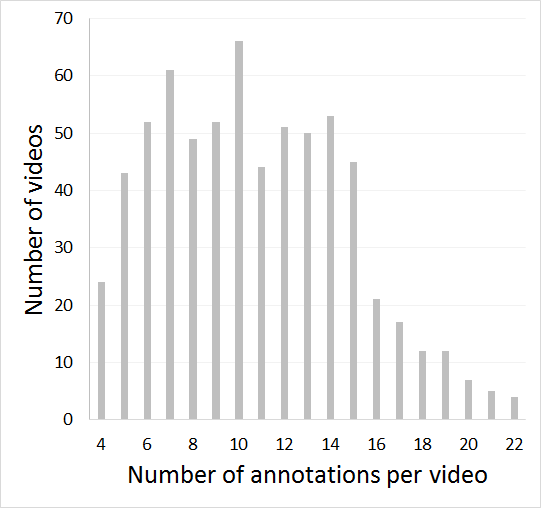
\includegraphics[width=\columnwidth]{figures/histogram_nb_sequences_for_nb_of_annotations.png}
	\caption{\label{fig:nb_annotations_per_sequence}Nb of sequences for each possible nb of annotations per sequence (>=3).}
\end{figure}

%figure Rank corr for Isola et al. et han et al., pour montrer que le nombre d'annotation sva plus vite pour les videos (mais crowdsourcing vs. laboratoire -- et autres facteurs...)

%%%%%%%%%%%%%%%%%%%%%%%%%%%%%%%%%%%%%
\subsection{Consistency analysis}
We implemented the method proposed in \cite{isola_2014_makes} to measure the human consistency. It answers the question: "Are the videos that are more memorable (or forgettable) for a group of observers also more likely to be remembered (or forgotten) by a different group of observers? The figure \ref{fig:human_consistency} presents the curve of the human consistency for each video sequence. It answers the question: "How many annotations for each do we need for the human consistency stop varying?'

%Curve of human consistency
\begin{figure}[!htbp]
	\centering
	\subfloat[(a) Human concistency for images in \cite{khosla_2015_understanding}]{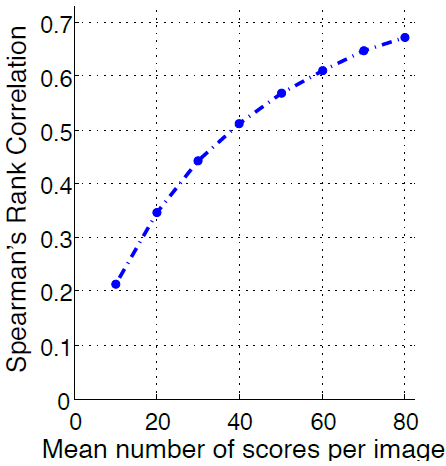
\includegraphics[width=0.3\columnwidth]{figures/human_consistency_LaMem.png}}
	\quad
	\subfloat[(b) Human consistency for videos for us]{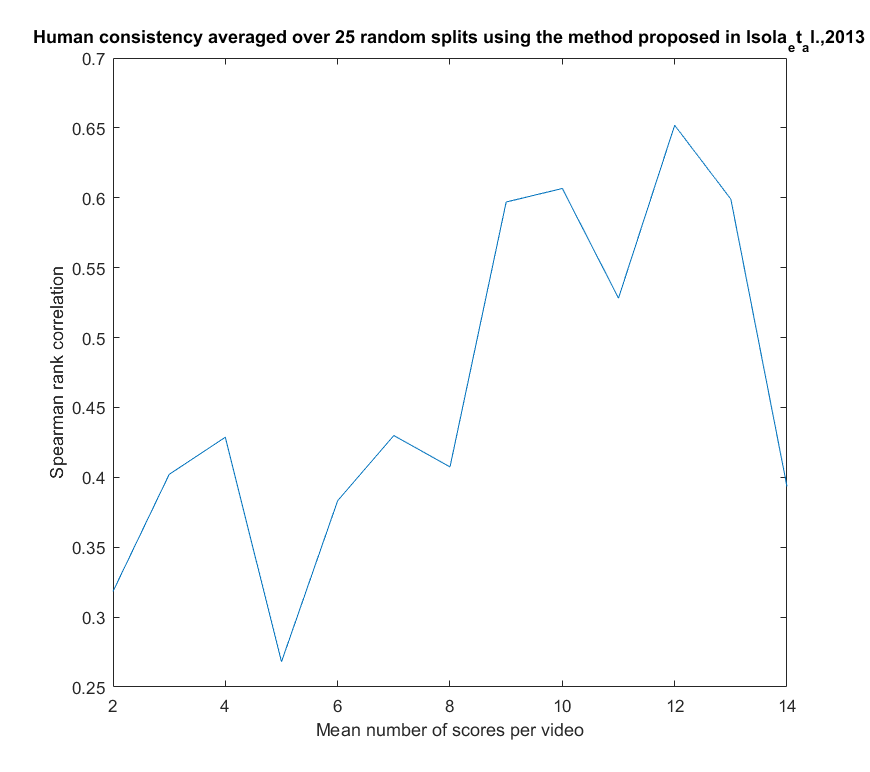
\includegraphics[width=0.3\columnwidth]{figures/human_consistency_nb_annotations.png}}
	\caption{\label{fig:human_consistency}Human consistency averaged over 25 random splits (right) obtained using the method proposed by \cite{isola_2014_makes}.}
\end{figure}

This curve show us that from 14 annotations (using our method) video memorability data has enough consistency

Individual and contextual differences, besides mandatory random variability, explain the $1-.65$ part of the memorability that is not universally derivable from the intrinsic informations of the videos.  

%Compare our and Khosla et al. curve dire que -- video + non-crowdsourcing + "real" long-term memory -- explique qu'on obtient avec beaucoup moins d'annotation la même human congruency.
If we compare the curve obtained by \cite{khosla_2015_understanding} (\ref{fig:human_consistency}(a))and the curve we obtained (b), we can note than we attain human consistency far more quickly than Khosla \textit{et al.}. At least three arguments go in the way of this results. First, we work with videos and they work with images ; maybe video memorability is more universal than image memorability because of the higher length of this kind of stimulus (but We can also note that the maximum human consistency is close for images and videos!!). Second, we obtain a measure of real long term memorability, and not a memorability measured some minutes after encoding step ; maybe this measure more representative of what is really memorable. Finally, we can advance the fact that in-lab experiment enable to obtain better memorability measure than crowdsourcing one, resulting to attain maximum human consistency earlier.

%%%%%%%%%%%%%%%%%%%%%%%%%%%%%%%%%%%%%
\subsection{Generic vs. Typical sequences}
% Tester s'il y a une différence entre les deux et en tirer des conséquence quant à leur validité --> How objective our measure of memorability is?

%%%%%%%%%%%%%%%%%%%%%%%%%%%%%%%%%%%%%
\subsection{Quality of the movies}
dvdrip vs. HD 720-1080 => Difference of memorability? => Interesting

%%%%%%%%%%%%%%%%%%%%%%%%%%%%%%%%%%%%%
\subsection{Response time}
%How to exploit the response time in the prediction models? --> two potential models for memorabilit prediction

The question here is: "Could we exploit response time to correct memorability score?"

We hypothesized that the most memorable the sequences, the faster the participant will answer.

%Memorability of sequence vs. their 
We observed a Person's correlation of $-0.35 (p<.0001)$ between the response time on the target and their memorability scores. This means that the videos with the higher memorability score tended to be answered fastly when correct detection by the participants, suggesting that a sequence most memorable is also a sequence for which we rapidly detect that it is memorable.

The global mean response time was $4.87 sec$ on targets and $5.96 sec$ on fillers.
A Student t-test for different sample size show a significant difference ($t(2836)=-5.34, p<.0001$). This means that the participants globally answered more rapidly for targets (i.e. correct detections) than for fillers (i.e. false alarm), probably because of their hesitation for fillers.

%%%%%%%%%%%%%%%%%%%%%%%%%%%%%%%%%%%%%
\subsection{Evolution of the memorability along time}
%Use order positions for that (e.g. mean memorability for position 1, 2... 120)





%%%%%%%%%%%%%%%%%%%%%%%%%%%%%%%%%%%%%
%tester la mémorability de séquences très proches (prise à intervalles très proche + vérif = même scène)

%indoor/outdorr comme isola et al. mais en contrecarrant l'effet de la couleur -- car ils espliquent que c'est par la corrrélation entre couleur et mémorabilité est expliqué par le fait que les couleurs plus froides sont d'exté.


%%%%%%%%%%%%%%%%%%%%%%%%%%%%%%%%%%%%%
\subsection{New manner to compute memorability scores: take into account time and FA}
%Une nouvelle manière pour prendre en compte les FA dans les scores de mémorabilité applicable à l'étude de la mémorabilité sur les images (si fonction : en parler dan sl'intro comme quoi les gens ne prennent jamais en compte les FA quoiqu'elles puissent être exploiter)
%Ce qui à la fin de cette section vient avant permet de conclure cette partie en disant : la meilleure façon de calculer les scores de mémorabilité, c'est comme ça.



%%%
\subsubsection{Participants' performance}
% The question here is: "Must we correct our memorabiliy scores by taking into account the mean memorability of the participants --> No, of the film --> No' --> So the point here is just to provide an overview.
The average memory performance was the following: the average percentage of correct detection was $48.2\%$ (SD of $14.1\%$) and the average percentage of false alarms was $4.78\%$ (SD of $5.63\%$).


%%%%%%%%%%%%%%%%%%%%%%%%%%%%%%%%%%%%%
\subsection{Logistic regression vs. SVM to personalize prediction model}
%Regression qui prend en compte tous les facteurs (voir ma thèse)
%See QoMEX paper to present the data

%We used the following factors:
	%Occidental/non-occidental, because the 100 movies are occidental (expept slumdog millionaires...)



%%%%%%%%%%%%%%%%%%%%%%%%%%%%%%%%%%%%%
% Other results possible
%%%%%%%%%%%%%%%%%%%%%%%%%%%%%%%%%%%%%
\subsection{Film genre and IMDB ratings}
%test the momorability od the sequences compare to the mean one of the movie.
%Correct bu the mean participant's performance
%And maybe other IMDB annotations/labels

\subsection{Context}
%Analyse the context (order of video presentation) influent the memo: to be check if we have enough information?
%Une vidéo par rapport à toutes les autres différentes à un impact sur sa mem ?
%S'inspirer de la technique de Bylinskii

\subsection{Features linked to memorability}
%tester ces features comme dans 'What makes a photograph...'
% Indoor/Outdoor, low-level visal feautures (color... -- i.e. as in isola et al.), salinecy maps

\subsection{Indoor \textit{.vs} outdoor scenes}



%add other relevant points found in MIT papers e.g.

%%%%%%%%%%%%%%%%%%%%%%%%%%%%%%%%%%%%%
\subsection{Memorability score calculation}
According to what was presented before in tis section, this is how we finally decided to compute our memorability scores...

%quality of the movies: dvdrip vs. HD 720-1080 => Difference of memorability? => Interesting


%%%%%%%%%%%%%%%%%%%%%%%%%%%%%%%%%%%%%%%%%%%%%%%%%%%%%%%%%%%%%%%%%%%%%%%%%%%%%%%%%%%%%%%%%%%%%%%%%%%%%%%%%%%%%%%%%%%%%%%%%%%%%%%%%%%%%%%%%%%%%%%%%%%%%%%%%
\section{MEMORABILITY PREDICTION} %for Khartik
%%%%%%%%%%%%%%%%%%%%%%%%%%%%%%%%%%%%%%%%%%%%%%%%%%%%%%%%%%%%%%%%%%%%%%%%%%%%%%%%%%%%%%%%%%%%%%%%%%%%%%%%%%%%%%%%%%%%%%%%%%%%%%%%%%%%%%%%%%%%%%%%%%%%%%%%%
%we used Soundnet...
% Nous construisons actuellement une base de données de grande ampleur avec une mesure purement objective de la mémoire.


%%%%%%%%%%%%%%%%%%%%%%%%%%%%%%%%%%%%%%%%%%%%%%%%%%%%%%%%%%%%%%%%%%%%%%%%%%%%%%%%%%%%%%%%%%%%%%%%%%%%%%%%%%%%%%%%%%%%%%%%%%%%%%%%%%%%%%%%%%%%%%%%%%%%%%%%%
\section{DISCUSSION}
%%%%%%%%%%%%%%%%%%%%%%%%%%%%%%%%%%%%%%%%%%%%%%%%%%%%%%%%%%%%%%%%%%%%%%%%%%%%%%%%%%%%%%%%%%%%%%%%%%%%%%%%%%%%%%%%%%%%%%%%%%%%%%%%%%%%%%%%%%%%%%%%%%%%%%%%%
%cite QooMEX for personlization of memorability model

%D'abord, le test de mémoire interroge une mémoire de vidéos vues longtemps (en moyenne, probablement plusieurs mois ou années) auparavant.



%file to make the data + movies names available.


%%%%%%%%%%%%%%%%%%%%%%%%%%%%%%%%%%%%%%%%%%%%%%%%%%%%%%%%%%%%%%%%%%%%%%%%%%%%%%%%%%%%%%%%%%%%%%%%%%%%%%%%%%%%%%%%%%%%%%%%%%%%%%%%%%%%%%%%%%%%%%%%%%%%%%%%%
\section{CONCLUSIONS}
%%%%%%%%%%%%%%%%%%%%%%%%%%%%%%%%%%%%%%%%%%%%%%%%%%%%%%%%%%%%%%%%%%%%%%%%%%%%%%%%%%%%%%%%%%%%%%%%%%%%%%%%%%%%%%%%%%%%%%%%%%%%%%%%%%%%%%%%%%%%%%%%%%%%%%%%%
% A conclusion section is not required. Although a conclusion may review the main points of the paper, do not replicate the abstract as the conclusion. A conclusion might elaborate on the importance of the work or suggest applications and extensions. 

%%%
 %Liste des features (comme/ceux de MediaEval 2015 à donner au téléchargement avec le début en sec de nos sequences)
 %Release text file for movie title, start/end time + features






\addtolength{\textheight}{-12cm}   % This command serves to balance the column lengths
                                  % on the last page of the document manually. It shortens
                                  % the textheight of the last page by a suitable amount.
                                  % This command does not take effect until the next page
                                  % so it should come on the page before the last. Make
                                  % sure that you do not shorten the textheight too much.


%%%%%%%%%%%%%%%%%%%%%%%%%%%%%%%%%%%%%%%%%%%%%%%%%%%%%%%%%%%%%%%%%%%%%%%%%%%%%%%%%%%%%%%%%%%%%%%%%%%%%%%%%%%%%%%%%%%%%%%%%%%%%%%%%%%%%%%%%%%%%%%%%%%%%%%%%
\section*{APPENDIX}
%%%%%%%%%%%%%%%%%%%%%%%%%%%%%%%%%%%%%%%%%%%%%%%%%%%%%%%%%%%%%%%%%%%%%%%%%%%%%%%%%%%%%%%%%%%%%%%%%%%%%%%%%%%%%%%%%%%%%%%%%%%%%%%%%%%%%%%%%%%%%%%%%%%%%%%%%
%Appendixes should appear before the acknowledgment.

%%%%%%%%%%%%%%%%%%%%%%%%%%%%%%%%%%%%%%%%%%%%%%%%%%%%%%%%%%%%%%%%%%%%%%%%%%%%%%%%%%%%%%%%%%%%%%%%%%%%%%%%%%%%%%%%%%%%%%%%%%%%%%%%%%%%%%%%%%%%%%%%%%%%%%%%%
\section*{ACKNOWLEDGMENT}
%%%%%%%%%%%%%%%%%%%%%%%%%%%%%%%%%%%%%%%%%%%%%%%%%%%%%%%%%%%%%%%%%%%%%%%%%%%%%%%%%%%%%%%%%%%%%%%%%%%%%%%%%%%%%%%%%%%%%%%%%%%%%%%%%%%%%%%%%%%%%%%%%%%%%%%%%
%This section is optional; it is a location for you
%to acknowledge grants, funding, editing assistance and
%what have you.

%%%%%%%%%%%%%%%%%%%%%%%%%%%%%%%%%%%%%%%%%%%%%%%%%%%%%%%%%%%%%%%%%%%%%%%%%%%%%%%%%%%%%%%%%%%%%%%%%%%%%%%%%%%%%%%%%%%%%%%%%%%%%%%%%%%%%%%%%%%%%%%%%%%%%%%%%
%% BIBLIOGRAPHY
%%%%%%%%%%%%%%%%%%%%%%%%%%%%%%%%%%%%%%%%%%%%%%%%%%%%%%%%%%%%%%%%%%%%%%%%%%%%%%%%%%%%%%%%%%%%%%%%%%%%%%%%%%%%%%%%%%%%%%%%%%%%%%%%%%%%%%%%%%%%%%%%%%%%%%%%%
\bibliographystyle{ACM-Reference-Format}
\bibliography{references} 

%%%%%%%%%%%%%%%%%%%%%%%%%%%%%%%%%%%%%%%%%%%%%%%%%%%%%%%%%%%%%%%%%%%%%%%%%%%%%%%%%%%%%%%%%%%%%%%%%%%%%%%%%%%%%%%%%%%%%%%%%%%%%%%%%%%%%%%%%%%%%%%%%%%%%%%%%
\end{document}